\section{\sys-PIM 上的 Attention 加速}
\label{sec:design-dp}

\begin{figure*}[t]
  \setlength{\abovecaptionskip}{-5pt}
  \setlength{\belowcaptionskip}{-10pt}
  \centering
  \begin{minipage}[t]{0.95\linewidth}
    \centering
    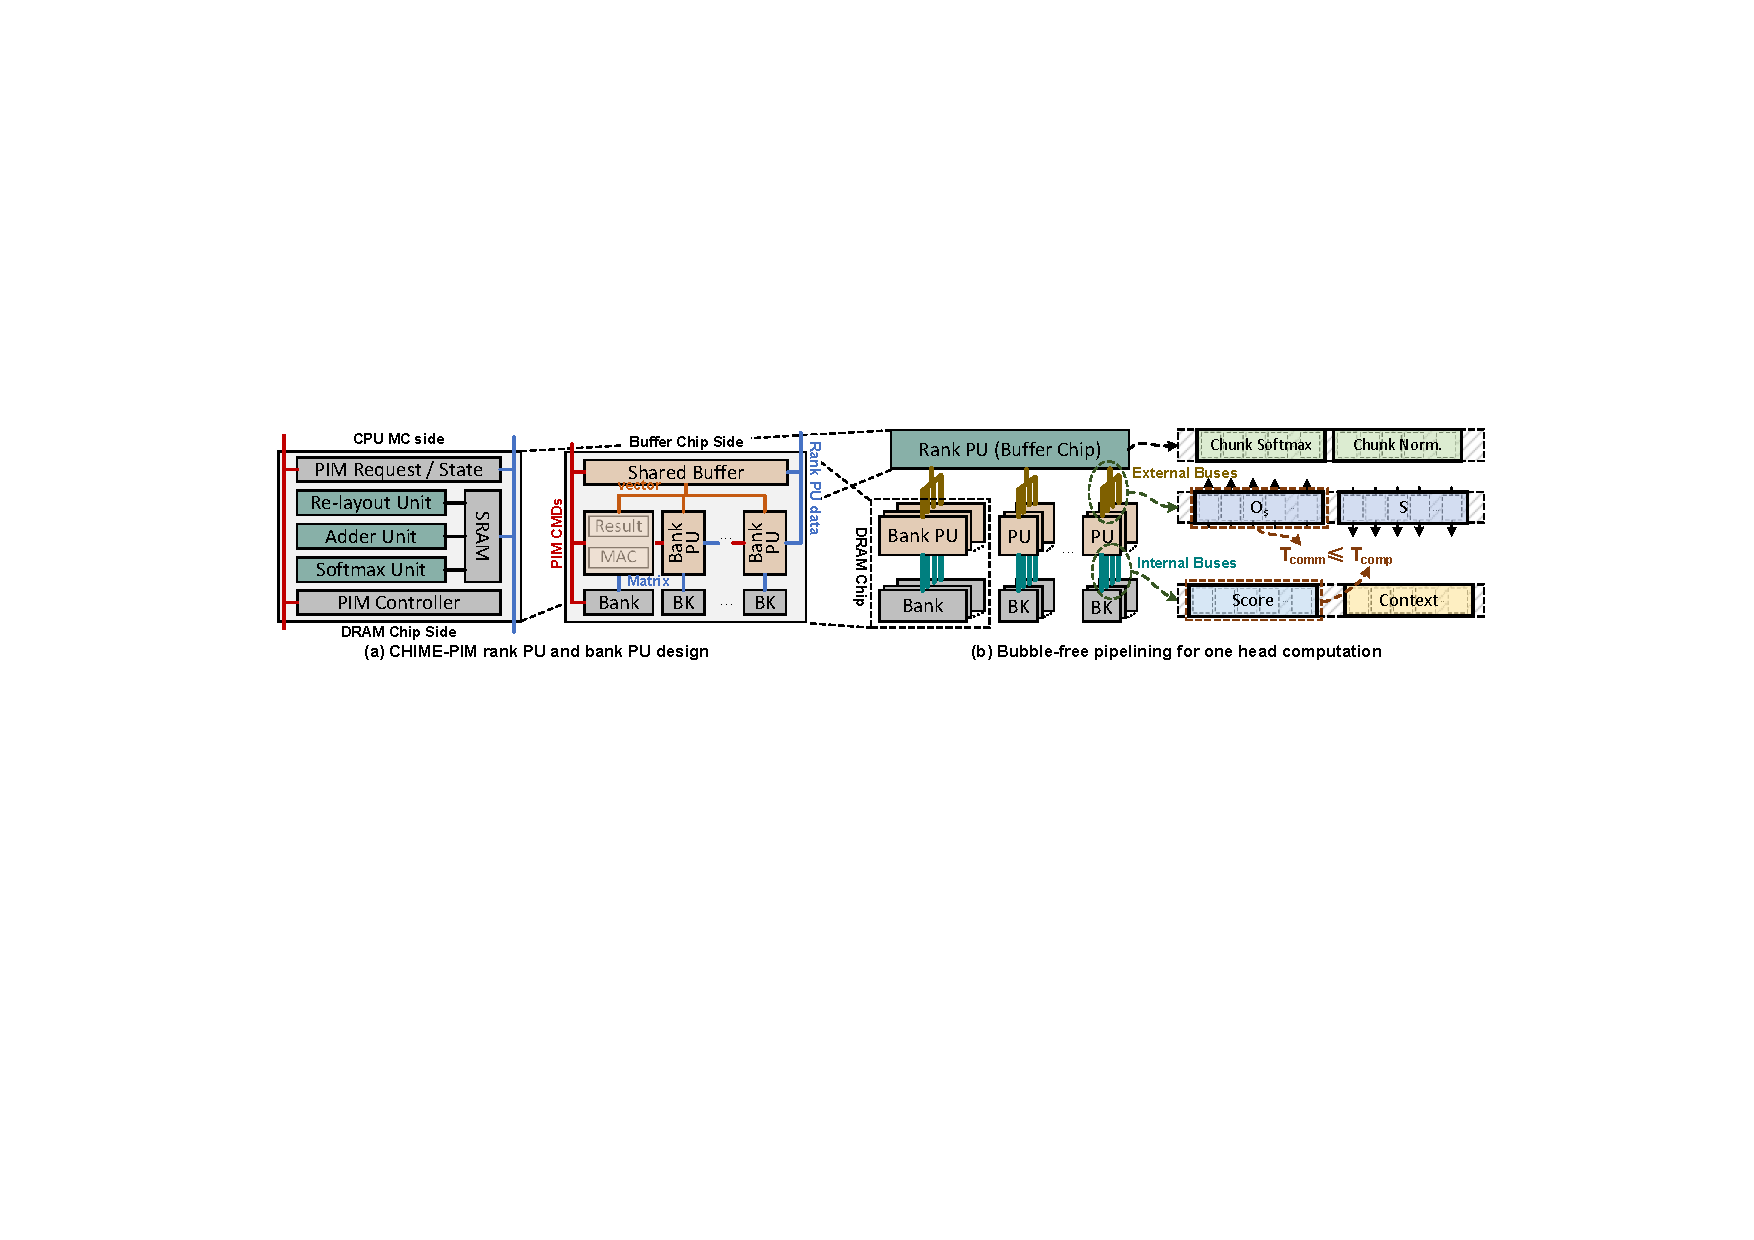
\includegraphics[width=\textwidth]{figs/design_arch_pipeline.pdf}
    \footnotesize
  \end{minipage}
  \caption{\textbf{采用无气泡流水线的 \sys-PIM 设计。}}
  \label{fig:design_arch_pipe}
\end{figure*}

本节介绍 \sys-PIM，这是一种面向高效 Attention 计算的新型 DIMM-PIM 硬件设计。

\myparagraph{硬件组件。}
如图~\ref{fig:design_arch_pipe}-a 所示，\sys-PIM 在 Bank 和 Rank 两个层级集成相互协作的处理单元（PU）。
Bank PU 采用 DRAM 工艺集成在 DRAM Bank 附近，从 Bank 中读取 KV cache 并执行 Score 与 Context 计算；共享缓冲区则用于向所有 Bank PU 广播输入向量。
所有 DRAM 芯片中的 Bank PU 并发执行乘加（MAC）操作，并将输出写入结果缓冲区。
Softmax 单元、加法器单元和重布局单元采用逻辑工艺集成在缓冲芯片上，作为 Rank PU 的一部分，能够与 Bank PU 异步执行。

\sys-PIM 的工作流无需修改主机 CPU 内存控制器，具体如下。
首先，CPU 通过普通写操作把 PIM 请求卸载到 Rank PU，后者进一步将其解码为 PIM 命令。
随后，专用 PIM 控制器经标准 DDR 接口向 DRAM 芯片发出 PIM 命令，以触发相应操作。
PIM 命令包括用于元数据设置和数据移动的命令，其中若干关键命令如下。
\texttt{PIM\_WR\_R} 将必要信息写入寄存器，例如计算范式（加法树或累加器）的配置、缓冲区自增索引机制等。
\texttt{PIM\_LD\_SB} 从特定 Bank 把数据加载到共享缓冲区，\texttt{PIM\_WR\_SB} 则把 Rank PU 中的数据写入共享缓冲区。
\texttt{PIM\_MAC} 在从 DRAM Cell 和共享缓冲区读取所需数据的同时，在所有 Bank 中执行 MAC 操作。
\texttt{PIM\_RD\_RB} 将所有 Bank 的结果缓冲区数据加载到 Rank PU。

\subsection{无气泡流水线}
为消除 Attention 计算中的数据同步开销，关键在于利用 DIMM-PIM 的独特架构，设计一种用计算隐藏通信的流水化 Attention 执行方式。
此外，我们通过定量分析和定制的 Head 映射方法，确保通信成本被完全隐藏。

\myparagraph{使用解耦内存总线与算子融合编排流水线。}
基于两项架构观察，我们为 PIM 中的 Attention 算子编排一种积极重叠计算与通信的流水化执行方式。
第一，内部内存总线（用于 Bank PU 访问 Bank）与外部内存总线（用于 Rank PU 访问 Bank PU 或共享缓冲区）可以解耦~\cite{chen2025asyncdimm}；如图~\ref{fig:design_arch_pipe}-b 所示，这使 Bank PU 上的计算算子与 Rank PU 发起或接收的数据传输能够同时执行。
第二，受 FlashAttention 算子融合技术~\cite{dao2022flashatten}（将 Attention 划分为分块 Tile 计算）的启发，我们编排细粒度算子流水线，在限制 Rank PU 上中间 Head 数据占用的同时最大化并发度。

具体而言，在 Score 阶段，每个 Bank PU 计算某个 Token 对应的输出 $O_s$ 并将其暂存在本地结果缓冲区后，Rank PU 会立即利用原本空闲的外部总线取回该输出。
我们的 Attention 算子以分块 Tile 为粒度运行；每个数据块由单个 Head 在一个或多个 Bank PU 上并行产生的数据构成。
数据在加法器单元中累加后，Softmax 单元逐块执行 Softmax。
这样一来，Score 与 Softmax 计算便可在 Bank PU 与 Rank PU 之间以数据块为单位形成流水线。
处理完所有 Token 后，最终的跨块归一化过程生成全局正确的 Softmax 输出 $S$，该过程同样以流式、逐块方式执行。
因此，最终 $S$ 元素的计算、将 $S$ 写回 DRAM 芯片的通信，以及后续 Context 计算可以组成流水线。

\myparagraph{通过定量分析与特定 Head 映射实现无气泡执行。}
\label{sec:design-dp-pipeline}
由于 DIMM 由多个相互协作的 DRAM 芯片组成一个 Rank，KV 矩阵（cache）及其计算会分布在这些 DRAM 芯片上。
这会增加缓冲芯片与 DRAM 芯片之间的数据传输量，本文称之为跨芯片数据传输。
即使跨芯片传输与 Bank PU 执行发生重叠，受 Rank PU 带宽限制，其开销仍可能在流水线执行中产生气泡并成为瓶颈。
为应对这一问题，我们首先结合 LLM 模型配置、硬件参数及 Head 映射方法，对跨芯片数据传输成本进行量化。
随后，我们使用特定 Head 映射方法实现无气泡流水线。
下述分析以单个 Head 的 Score 计算为例，Context 计算可以采用类似分析。

传输 Score 输出 $O_s$ 的开销记为 $T_{comm}$，满足 $T_{comm}={N_{comm}}/{B_{comm}}$；其中 $N_{comm}$ 为跨芯片数据传输量，$B_{comm}$ 为相应带宽。
具体而言：
\begin{align*}
  {N_{comm}}={L_t}\times{N_{gqa}}\times{N_{hc}}, \qquad
  {B_{comm}}=({B_{rk}}\times{N_{hc}})/N_{chips}
\end{align*}
其中，$L_t$ 为 Token 长度，$N_{gqa}$ 为 GQA 组大小，$N_{hc}$ 为分配给该 Head 的芯片数，$B_{rk}$ 为 Rank 带宽，$N_{chips}$ 为一个 Rank 中的 DRAM 芯片总数。
因此，通信时间为：
\begin{align*}
  {T_{comm}}=({L_t}\times{N_{gqa}}\times{N_{chips}})/{B_{rk}}
\end{align*}
这意味着 DIMM 的分布式芯片可能引入额外 $N_{chips}\times$ 的数据传输开销，而 GQA 组大小会进一步加剧该开销。

采用流水化执行后，实现无气泡重叠的关键是 $T_{comm}\le T_{comp}$，即 Bank PU 的计算可以完全覆盖传输。
$T_{comp}$ 可由 $T_{comp}={N_{comp}}/{B_{comp}}$ 计算，其中 $N_{comp}$ 为 Bank PU 读取的数据量（K Cache），$B_{comp}$ 为 Bank PU 的聚合带宽。
具体而言：
\begin{align*}
  {N_{comp}}={L_t}\times{E_h}\times\left\lceil {N_{gqa}}/{N_{cmr}} \right\rceil, \qquad
  {B_{comp}}={B_{bk}}\times{N_{bk}}\times{N_{hc}}
\end{align*}
其中，$E_h$ 为 Head 嵌入维度，$B_{bk}$ 为 Bank PU 带宽，$N_{bk}$ 为 Bank 数量，$N_{cmr}$ 表示 Bank PU 中算术单元的计算--内存比。
一般而言，$N_{cmr}=1$ 可最大化 MHA 计算的带宽利用率，而对 GQA-8 计算采用 $N_{cmr}=8$~\cite{park2024attacc}。
因此，计算时间为：
\begin{align*}
  {T_{comp}}=({L_t}\times{E_h}\times\left\lceil {N_{gqa}}/{N_{cmr}} \right\rceil)/({B_{bk}}\times{N_{bk}}\times{N_{hc}})
\end{align*}

综合考虑 $T_{comm}$ 与 $T_{comp}$，确保无气泡的关键条件 $T_{comm}\le T_{comp}$ 可写为：
\begin{align*}
  \frac{{L_t}\times{N_{gqa}}\times{N_{chips}}}{{B_{rk}}}
  \le
  \frac{{L_t}\times{E_h}\times\left\lceil {N_{gqa}}/{N_{cmr}} \right\rceil}{{B_{bk}}\times{N_{bk}}\times{N_{hc}}}
\end{align*}

我们发现，在模型与硬件配置给定时，Head 映射方式（$N_{hc}$）是满足该不等式时唯一可调的变量。
因此，Head 映射需满足：
\begin{align}
  \label{equ:head-mapping}
  N_{hc} \le \frac{E_h \times B_{rk}\times \left\lceil {N_{gqa}}/{N_{cmr}} \right\rceil}{B_{bk} \times N_{bk} \times N_{gqa} \times N_{chips}}
\end{align}

以表~\ref{tab:simulator} 和表~\ref{tab:model} 的配置为例，对于 MHA（$N_{gqa}=1$），系统要求 ${N_{hc}}\le 8$；对于 GQA-8（$N_{gqa}=8$），则要求 ${N_{hc}}\le 1$。
本文对 MHA 采用 $N_{hc}=8$，对 GQA-8 采用 $N_{hc}=1$；这是因为将一个 Head 映射到更多芯片有望简化 Rank 级负载均衡，使模型中的 Head 能够映射到更多 Rank。

\begin{figure}[t]
  \setlength{\abovecaptionskip}{5pt}
  \setlength{\belowcaptionskip}{-10pt}
  \centering
  \begin{minipage}[t]{\linewidth}
    \centering
    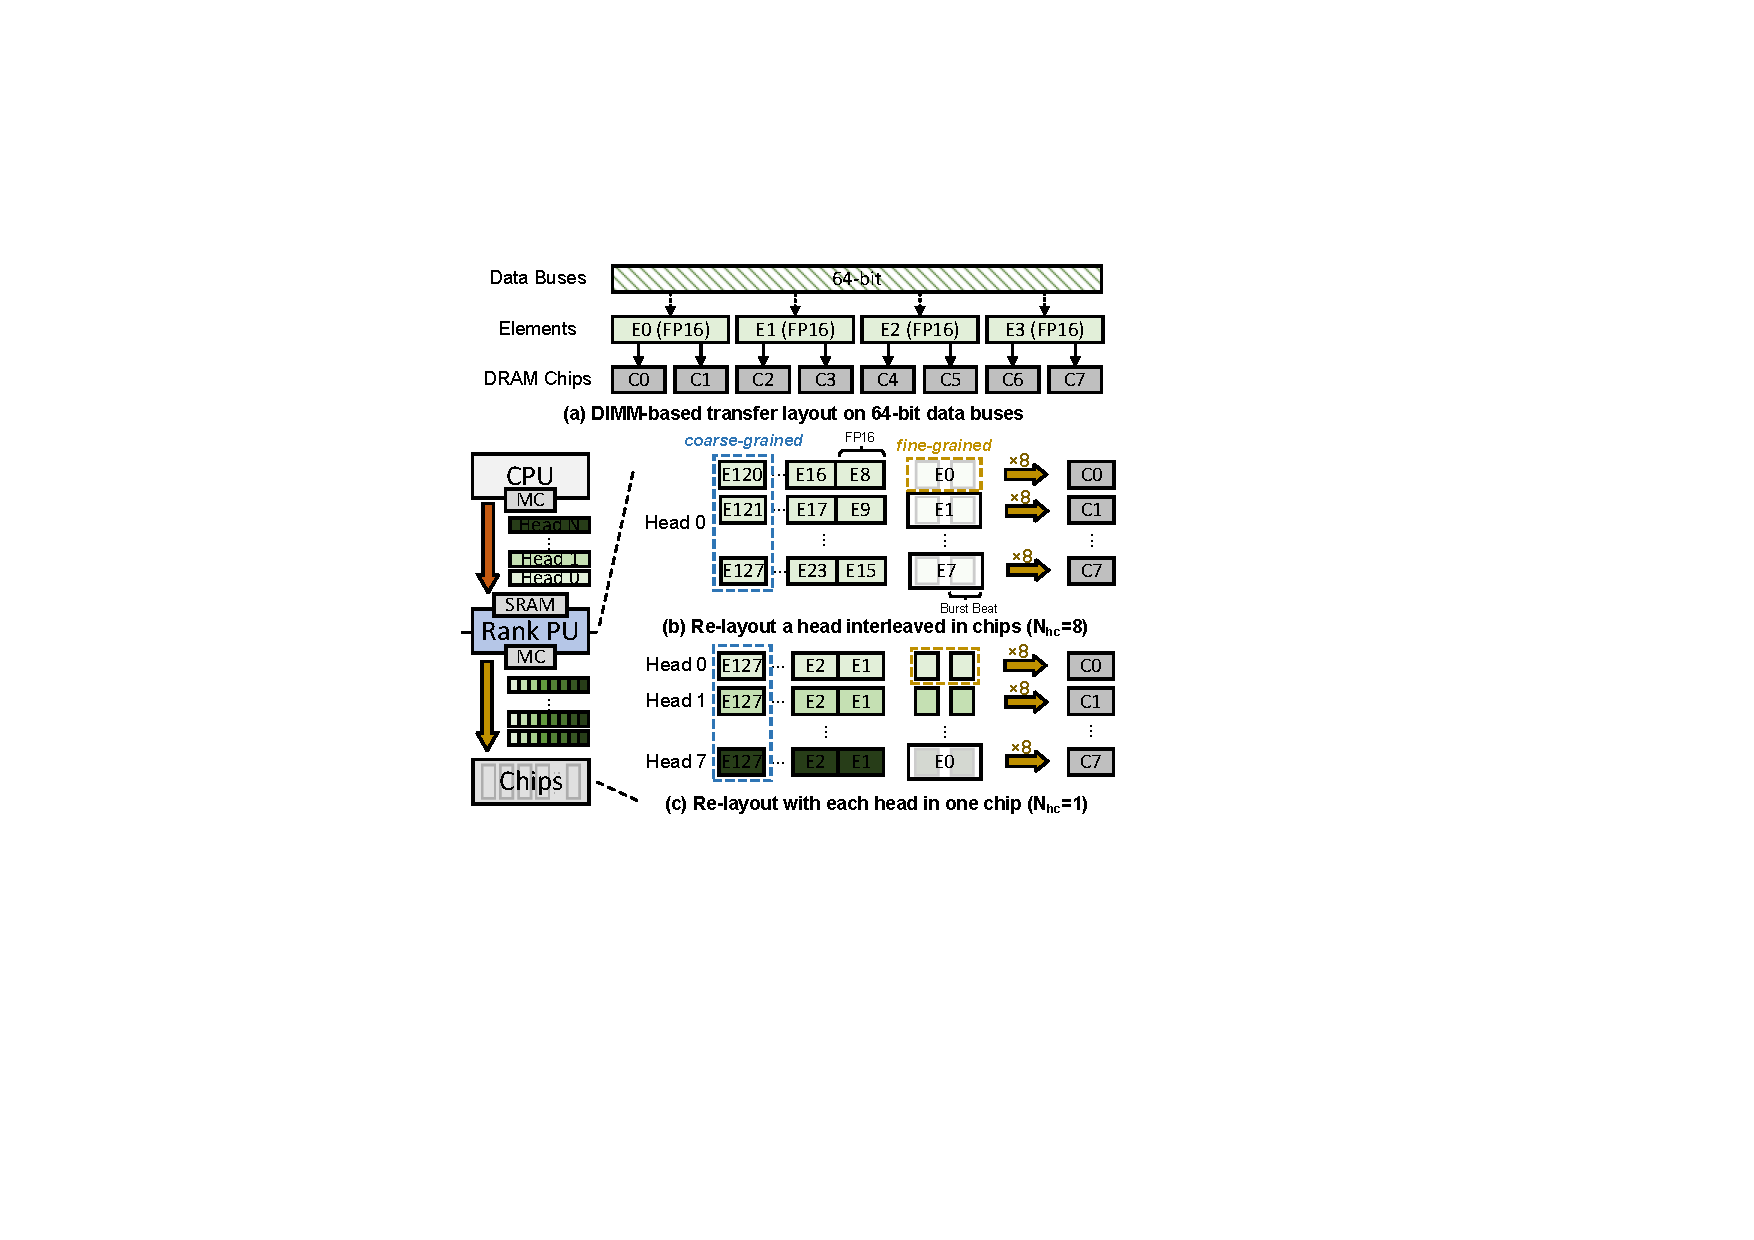
\includegraphics[width=\textwidth]{figs/design-arch-relayout.pdf}
    \footnotesize
  \end{minipage}
  \caption{\textbf{以 8$\times$8 芯片为例的混合粒度重布局。}
  \textit{E0--E127：一个 Head 中的元素 0--127；C0--C7：DRAM 芯片 0--7。}}
  \label{fig:design_arch_relayout}
\end{figure}

\subsection{混合粒度重布局}
\label{sec:design-dp-relayout}
除了特定 Head 映射布局之外，包含分布式 DRAM 芯片的 DIMM 还会约束元素布局，如图~\ref{fig:design_arch_relayout}-a 所示。
为在数据总线上连续传输，单个元素可能跨越多个 DRAM 芯片（例如，一个 FP16 元素跨两个 $\times$8 芯片），这从根本上阻止了 PIM 执行。
以往由 CPU 辅助的重布局方案~\cite{devaux2019true,kim2021gradpim,asghari2016chameleon,lee2024pimmmu,gomez2022benchmarking}需要反复访问内存，产生不可忽略的开销（第~\ref{sec:eval-ablation} 节）。
为解决这一问题，我们提出\emph{混合粒度重布局}：利用 Rank PU 的重布局单元，在通信过程中进行在线数据变换。

图~\ref{fig:design_arch_relayout} 左侧以数据卸载为例展示了重布局过程。
QKV 向量首先缓存在 Rank PU 的片上 SRAM 中，而不是直接写入 DRAM Bank。
完成重布局后，向量才被存入 DRAM 芯片。
重布局单元分别通过细粒度与粗粒度重布局来解决元素映射和 Head 映射不匹配问题。
第一，在细粒度重布局中，重布局单元确保每个元素完整驻留在单个芯片上。
如图~\ref{fig:design_arch_relayout} 所示，单个元素的各比特被排列到连续的突发拍（burst beat）中，以存入一个芯片（棕色虚线框）。
例如，元素 0（E0）的 16 个比特在两个连续突发拍（位于同一次 DDR 突发传输中）内传输，因而存入芯片 0（C0）。
第二，在粗粒度重布局中，重布局单元把每个 Head 映射到 $N_{hc}$ 个芯片。
来自一定数量 Head 的元素会一同调度，以遵循 Head 映射（蓝色虚线框）。
例如，在图~\ref{fig:design_arch_relayout}-b 的 $N_{hc}=8$ 情况下，重布局后每个突发拍包含来自单个 Head 的元素，因此一个 Head 被传输到 8 个芯片。
在图~\ref{fig:design_arch_relayout}-c 中，来自 8 个 Head 的元素置于一个突发拍中，因此每个 Head 只传输到单个芯片。
数据载回时，重布局执行逆向过程。
